\begin{figure}[htbp]\centering
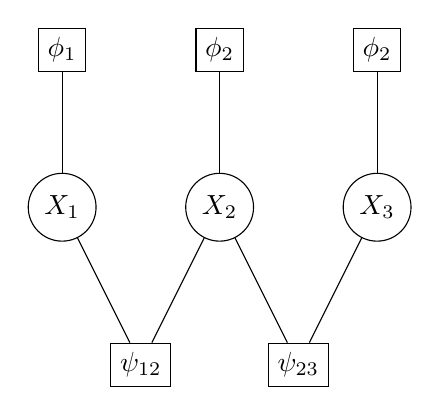
\begin{tikzpicture}[var/.style={circle,draw},factor/.style={rectangle,draw}]
\node[var] (x1) at (0,0) {$X_1$}; 
\node[var] (x2) at (2,0) {$X_2$};
\node[var] (x3) at (4,0) {$X_3$};
\node[factor] (u1) at (0,2) {$\phi_1$};
\node[factor] (u2) at (2,2) {$\phi_2$};
\node[factor] (u3) at (4,2) {$\phi_2$};
\node[factor] (p12) at (1,-2) {$\psi_{12}$};
\node[factor] (p23) at (3,-2) {$\psi_{23}$};
\path (x1) edge (u1); \path (x2) edge (u2); \path (x3) edge (u3);
\path (x1) edge (p12); \path (x2) edge (p12);
\path (x2) edge (p23); \path (x3) edge (p23);
\end{tikzpicture}\caption{Simple factor graph with $3$ variables, unary and pairwise factors.}
\end{figure}